\documentclass[../../Problems]{subfiles}
\begin{document}
\subsection{Schr\"oder Number}{\label{pp:schrodernumber}}
A Schroder Number is count of \hyperref[pp:delannoynumber]{Delannoy Walks} ($m=n$) when the path always stays \emph{on or below the diagonal}.
\begin{figure}[H]
	\centering
	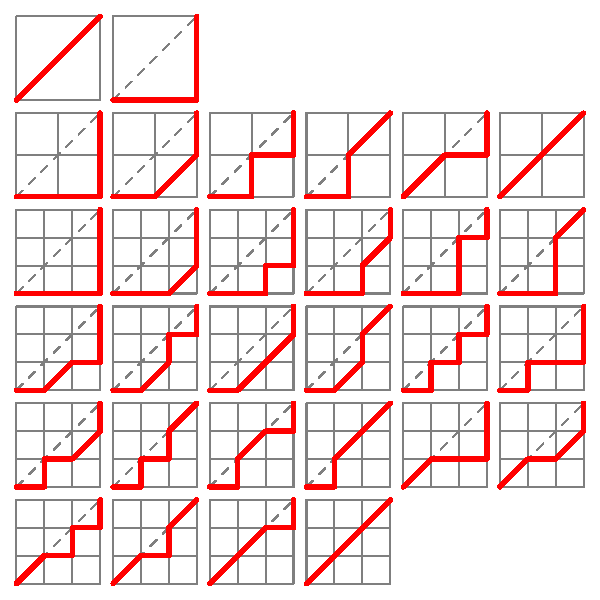
\includegraphics[width = 0.32\linewidth]{Schroder Number.pdf}
	\caption{Example walks for case $n=1\ (\#2),\ n=2\ (\#6),\ n=3\ (\#22)$ (\href{https://mathworld.wolfram.com/SchroederNumber.html}{Image Source})}
	\label{fig:schrodernumber}
\end{figure}
\vspace{-1.5em}
\textbf{Problem Statement:}\\
Find the \emph{Schroder Number} for a given $n$ (for all test cases).
\begin{testcasesFunction}
	{$t$ \hfill(number of test cases, an integer)\\
	$n_1\ n_2\ \ldots n_t$ \hfill($t$ space seperated integers for each testcase)}
	{Number of Schroder Numbers for $n_i$  \hfill(each test case on a newline)}
	{$1 \leq n_i \leq 14$}
	{\texttt{int schroder\_number(int n)} -- returns the number of possible delannoy walks for $n$.}
	{14\\1 2 3 4 5 6 7 8 9 10 11 12 13 14}
	{2\\6\\22\\90\\394\\1806\\8558\\41586\\206098\\1037718\\5293446\\27297738\\142078746\\745387038}
	{https://github.com/paramrathour/CS-101/tree/main/Starter Codes/Schroder Number.cpp}
\end{testcasesFunction}
\end{document}